\section{Predictive approach}
\label{predictive-approach}
Under highly variable input rate environments, input prediction is crucial in order to adapt the system processing logic over the time, which will keep events flowing, ensuring accurate results.

In our second proposal, denoted  \pSPS{}, we use a prediction model for the estimation of the optimal number of replicas for a given operator in the DAG. Therefore, unlike \rSPS{}, a reactive approach that focuses on detecting traffic peaks, \pSPS{}, a predictive approach, focuses on finding patterns in the traffic, predicting possible overloads or underloads.

Table~\ref{tab:notations} summarizes all the parameter's notations used in \pSPS{}. 

\begin{table}[!ht]
\begin{tabular}{|c|l|}
    \hline
    \textit{\textbf{Parameter}}     & \textit{\textbf{Description}}             \\  \hline
    $O_i$                           & operator $i$ \\
    $t$                             & time interval number \\ 
    $td$                            & time interval duration  \\
    $et_i$                          & average execution time of one event by $O_i$  \\
    $q_i(t)$                        & queue of events received and not processed by $O_i$ at the end of $t$ \\
    $\lambda_G(t)$                  & number of events sent by input data during $t$ \\
    $\lambda^r_i(t)$                & number of events received by $O_i$ during $t$\\
    $\lambda^p_i(t)$                & number of events received by $O_i$ sent from $O_p$ during $t$\\
    $\mu_i(t)$                      & number of events processed by $O_i$ during $t$\\
    $\theta_x(t)$                   & percentage of events processed of $\lambda_G(t)$ by $O_x$ during $t$\\
    $O_i^p$                         & predecessor operator of $O_i$ in the SPS DAG \\
    $\theta_i^p(t)$                 & percentage of events produced by $O_i^p$ sent to $O_i$ during $t$\\
    $\widehat{\lambda_G}(t+1)$      & predicted number of events sent by input data during $t+1$ \\
    $\widehat{\lambda_i}(t+1)$      & predicted number of events to process by $O_i$ during $t+1$ \\
    $\widehat{\lambda_i^r}(t+1)$    & predicted number of events received by $O_i$ during $t+1$ \\
    $\widehat{\lambda_i^q}(t+1)$    & predicted number of queued events to  be processed by $O_i$ during $t+1$ \\
    $r_i(t+1)$                      & number of replicas of $O_i$ computed at the end of $t$  \\
    \hline
\end{tabular}
\caption{Parameters notation and their description in \pSPS{}.}
\label{tab:notations}
\end{table}

\subsection{Predictive model}
% REPLICAS
The aim of our predictive model is to estimate how many active replicas would be necessary for operator $O_i$ to process the number of input events for the next time interval $t+1$ ($\widehat{\lambda_i}(t+1)$). It considers the processing capacity of $O_i$ as the average execution time of one event at the operator ($et_i$). At the end of each interval, the number of replicas is calculated following Equation \ref{eq:prediction-replicas}.

\begin{equation}
    \label{eq:prediction-replicas}
    r_i(t+1) = \frac{\widehat{\lambda_i}(t+1) \times et_i}{td}\\
\end{equation}

Let us consider that the time interval duration ($td$) equals $1000~ms$. Figure \ref{fig:prediction-replicas} shows an example composed by three independent operators  ($O_1$, $O_2$, and $O_3$) which have different average execution time of one event ($et_i$).  At the beginning of $t$, all the three operators have two replicas ($r_i = 2$). And by prediction, they will receive the same number of events $\widehat{\lambda_i}(t+1)$. 

In this example, due to $et_i$'s differences, Equation \ref{eq:prediction-replicas} will render $r_1(t+1)=2$, $r_2(t+1)=1$, and $r_3(t+1)=4$ at the end of $t$. Such results inform that the number of $O_1$'s active replicas should not change but that of $O_2$ (resp., $O_3$) is overestimated (resp., underestimated) and should be reduced (resp., increased) to one (resp., four). 

\begin{figure}[!ht]
    \centering
    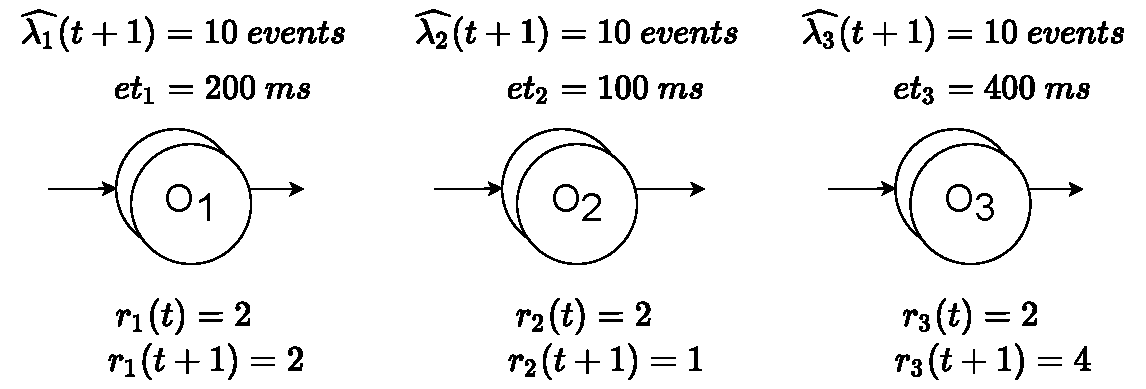
\includegraphics[width=0.9\textwidth]{figures/concepts/PA-SPS-PredictiveModel.pdf}
    \caption{Example of the number of replicas calculation, according Equation \ref{eq:prediction-replicas}.}
    \label{fig:prediction-replicas}
\end{figure}

We point out that since prediction of a number of active replicas depends on multiple factors, dynamically determining it is not trivial.
Thus, we model this complex problem so that the value of $\widehat{\lambda_i}(t+1)$ is determined by Equation \ref{eq:prediction-lambda} which, in turn, is determined by the prediction of received events ($\widehat{\lambda_i^r}(t+1)$) and the prediction of queued events ($\widehat{\lambda_i^q}(t+1)$) during the next time interval.

\begin{equation}
\label{eq:prediction-lambda}
    \widehat{\lambda_i}(t+1) = \widehat{\lambda_i^r}(t+1) + \widehat{\lambda_i^q}(t+1)
\end{equation}

% DEPENDECY (Domino Effect)
In most SPS, the processing logic is represented by a DAG. The latter establishes a dependency condition where operators share a stream of events according to their location in the DAG. For example, let's consider a linear DAG with two operators (see Figure \ref{fig:sps-dependence}), $O_1$ and $O_2$, and their respective values of $\lambda^r_i(t)$ and $\mu_i(t)$ (see Table \ref{tab:notations}). $\mu_1(t)$ and $\lambda^r_2(t)$ are equal since operator $O_1$ has sent all the events it has processed to its single successor $O_2$. If $i$ is the initial single DAG operator, then $\lambda^r_i(t)$ equals $\lambda_G(t)$ ($\lambda^r_1(t) = \lambda_G(t)$).

Note that the increase of $O_p$'s number of active replicas at the end of the interval $t$ has a direct impact in $O_p$'s successors, since, in this case, $\mu_p(t+1)$ increases and thus,  $\lambda^r_i(t+1)$ too, inducing a domino effect that the prediction formulations should avoid. For example, in Figure \ref{fig:sps-dependence}, if $\mu_1(t+1)$ increased from $5$ to $10$ events, due to the replication of $O_1$ at the end of $t$, $\lambda^r_2(t+1)$ would increase as well. Hence, if the operators process all received events during $t+1$, we have that $\lambda_G(t+1)=\lambda^r_1(t+1)=\mu_1(t+1)=\lambda^r_2(t+1)$ and, consequently, all operators $O_i$ are dependent on $\lambda_G(t)$. 

\begin{figure}[!ht]
    \centering
    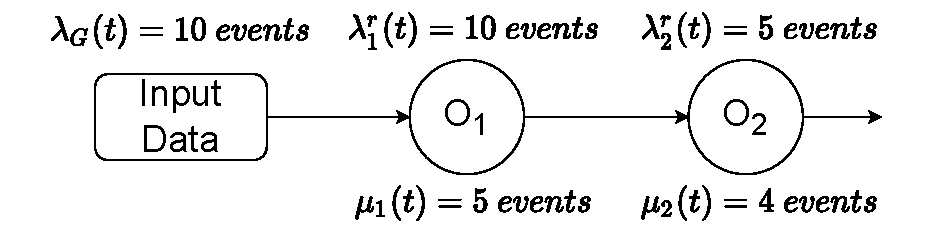
\includegraphics[width=0.8\textwidth]{figures/concepts/PA-SPS-Dependence.pdf}
    \caption{DAG operators dependence example.}
    \label{fig:sps-dependence}
\end{figure}


% PREDICTION INPUT
The above example is a borderline case. In a SPS DAG, not always, all the output processed events of $O_i^p$, the predecessor operator of $O_i$, will be sent to $O_i$. It might happen that $O_i^p$ splits, filters, or replicates the events into several streams, sending each of them to one of its different successor operators in the DAG. Thus, we define Equation \ref{eq:theta-predecessor}, where $\theta_i^p$ parameter tackles this issue by informing the percentage of processed events of $O_i^p$ sent to $O_i$.

\begin{equation}
  \label{eq:theta-predecessor}
  \theta_i^p(t) =  \frac{\lambda^p_i(t)}{\mu_p(t)}\\
\end{equation}

% THETA
Considering the condition of dependence among the operators, $\theta_{i}(t)$ is defined as the sum of the events processed by the predecessors of $O_i$, where it is determined by all the predecessor operators $O^p_i$ as presented in Equation \ref{eq:theta}. Note that $\theta_i(t)$ must be calculated from the initial operators.

\begin{equation}
  \label{eq:theta}
  \theta_i(t) =  \sum_{p \in pred(O_i)} \theta_i^p(t) \times \theta_p(t)\\
\end{equation}

Thus, we define Equation \ref{eq:prediction-input}, which predicts the number of events received by the operator $O_i$ during $t+1$. For its calculation, the percentage of events processed by operator $O_i$ is used ($\theta_i(t)$), according to the prediction of the number of events sent by the input data ($\widehat{\lambda_G}(t+1)$). Note that a predictive model is used to calculate $\widehat{\lambda_G}(t+1)$ (see Section \ref{psps-input-prediction}).

\begin{equation}
    \label{eq:prediction-input}
  \widehat{\lambda_i^r}(t+1) =  \widehat{\lambda_G}(t+1) \times \theta_i(t)\\
\end{equation}

Figure \ref{fig:prediction-input} shows a DAG example and $\theta_i^p$ value which was  estimated applying Equation \ref{eq:theta-predecessor}. It is worth pointing out that, given the dependence among the operators, it is necessary to start from the initial operator downstream to the last one. Since $\theta_1$ is equal to $1$, $O_1$ receives all the events sent from the input and then splits them among $O_2$ and $O_3$.  In this case, the two operators do not receive all the events from their respective predecessor, $O_1$; therefore $\theta_2$ and $\theta_3$ have values $0.7$ and $0.3$ respectively. Finally, operator $O_4$ receives events from its predecessor operators $O_2$ and $O_3$. However, $O_2$ does not send all its processed events to $O_4$, but only $\theta_4^2=0.4$, unlike $O_3$ which sends all processed events to $O_4$ ($\theta_4^2=1$). The value of $\theta_4$ is, therefore, $0.58$, according to Equation \ref{eq:theta}. 

\begin{figure}[!ht]
    \centering
    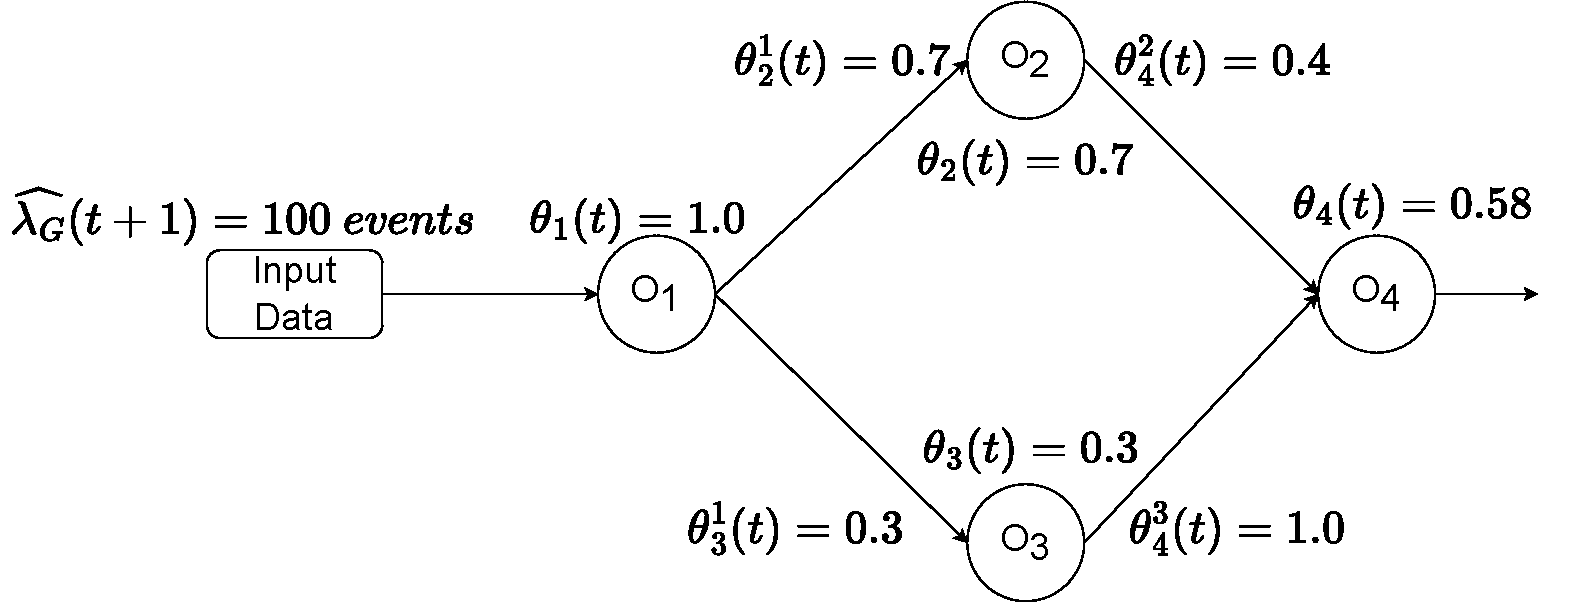
\includegraphics[width=1\textwidth]{figures/concepts/PA-SPS-PredictionInput.pdf}

    \vspace*{0.5cm}
    
    \begin{tabular}{c|c|c|c|c}
        & $O_1$ & $O_2$ & $O_3$ & $O_4$\\ \hline
        $\widehat{\lambda^r_i}(t+1)$ & 100 & 70 & 30 & 58
    \end{tabular}
    \caption{DAG example of predicted received number of events according to Equation \ref{eq:prediction-input}.}
    \label{fig:prediction-input}
\end{figure}

% QUEUE

Finally, we should consider the events received and not processed during $t$ by $O_i$ which are kept in $q_i(t)$. Hence, the number of input events $\widehat{\lambda_i}(t+1)$ that $O_i$ should actually process in $t$ is composed not only of received events $\widehat{\lambda_i^r}(t+1)$ but also of the events queued in $O_i$ and its predecessor operators $O^i_p$ because of the domino effect on the DAG.

For this reason, Equation \ref{eq:prediction-queue} is defined, where $\widehat{\lambda_i^q}(t+1)$ consists of the number of events queued in $O_i$ and the percentage of queued events that will be sent by its predecessor operators $O^p_i$ during $t+1$. Note that there is one queue per operator.

\begin{equation}
\label{eq:prediction-queue}
  \widehat{\lambda_i^q}(t+1) =  |q_i(t)| + \sum_{p \in pred(O_i)} \widehat{\lambda_p^q}(t+1) \times \theta_p(t)
\end{equation}


% INPUT PREDICTION
\subsection{Input prediction}
\label{psps-input-prediction}
As mentioned above, Equation \ref{eq:prediction-input} used $\widehat{\lambda_G}(t+1)$, which indicates the predicted number of events sent by the input data during $t+1$. Its prediction is based on the previous observation windows according to a number of samples $s$. The observation time interval is determined by $to$. The prediction is applied by one of the following models:

\begin{itemize}
    \item \textit{Basic}: considers that the input data values during $t+1$ will behave the same way as they did during $t$.
    \item \textit{LR}: uses a simple linear regression similar to the one presented in \citep{montgomery2021introduction}.
    \item \textit{FFT}: Fast Fourier Transform decomposes functions depending on space or time into functions depending on frequency. It allows to predict the input data by modeling its behavior as a time series \citep{nussbaumer1982fast}.
    \item \textit{ANN}: uses a neural network regression model, specifically a Multi-Layer Perceptron (MLP). It implements an MLP algorithm for training and testing data sets using backpropagation and stochastic gradient descent methods \citep{riedmiller2014multi}. The parameters values used in this model where extracted from \citep{PedregosaVGMTGBPWDVPCBPD11}.
    \item \textit{RF}: Random Forest combines learning methods with the decision tree framework to create multiple randomly drawn decision trees from the data. \citep{rigatti2017random}. The parameters used are the values for defects in \citep{PedregosaVGMTGBPWDVPCBPD11}.
\end{itemize}


\subsection{MAPE implementation}
As with the reactive approach, in \pSPS{} we will use the MAPE model for the automation of system adaptation. The big difference is in the \textit{Analysis} module, because it performs a request to the predictor model for input rate prediction. Figure \ref{fig:psps-mape} presents the
architecture of \pSPS{}:

\begin{figure}[!ht]
    \centering
    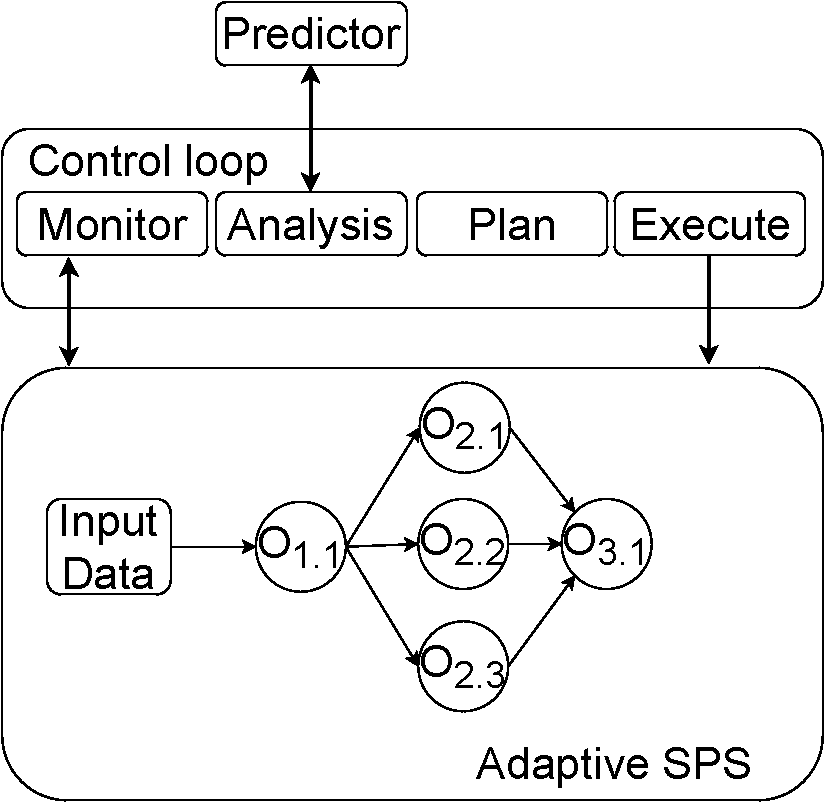
\includegraphics[width=0.45\textwidth]{figures/concepts/PA-SPS-Architecture.pdf}
    \caption{The architecture of \pSPS{}.}
    \label{fig:psps-mape}
\end{figure}

In our system, the MAPE model integrates the before-mentioned components where each of the four MAPE modules performs the following tasks: 
\begin{enumerate} 
    \item \textit{Monitor}: Module in charge of collecting statistics from the DAG. At a predefined time interval $t$, the monitor requests the values of $\lambda_i(t)$, $et_i$, and the number of queued events $q_i(t)$.
    \item \textit{Analysis}: The module analyses input data and predicts its behaviour following Equation \ref{eq:prediction-lambda}. Note that the analysis is performed for each operator in the DAG.
    \item \textit{Plan}: Based on the previous analysis, the \textit{Plan} module defines whether it is necessary or not to modify the system resource capacity. For this, we define Algorithm \ref{alg:psps-planning} which is explained in Section \ref{psps-planning}.  
    \item \textit{Execute}: Module in charge of carrying out the change in an operator's current number of replicas, if required by the \textit{Plan} module.
\end{enumerate}


\subsection{Planning}
\label{psps-planning}
Algorithm \ref{alg:psps-planning} presents the algorithm executed by the \textit{Plan} module for the $O_i$ operator, deciding if the number of replicas of $O_i$ should be increased (or decreased) by $k$ or remain the same.

First, the algorithm determines the number of replicas for the next time interval is computed (line 1). To this end, the number of necessary replicas is calculated according to Equation \ref{eq:prediction-replicas}, using an input data predictor to determine the future behaviour of the input stream. Then, the $getReplicas(O_i)$ function returns the current active replicas of $O_i$. Hence, the difference between the prediction and the current number of replicas will be the number of replicas ($k_i$) to be modified (line 2). If the value of $k$ is positive, then $k_i$ replicas are activated (line 4). If the value of $k$ is negative, then $k_i$ replicas are deactivated (line 6). If the value of $k$ is 0, then the same number of active replicas is kept.

\begin{algorithm}[!ht]
\caption{Adaptive planning algorithm according to the predictive approach for the operator $O_i$.}
 \begin{algorithmic}[1]
 	\REQUIRE Statistics Operator $O_i$ in time interval $t$.
 	\ENSURE Modifying the current number of active replicas of operator $O_i$.
	\STATE $r_i(t+1) \gets$ computeReplicas($\widehat{\lambda_i}(t+1)$ , $et_i$, $td$)
	\STATE $k_i \gets r_i(t+1)$ - getReplicas($O_i$)
	\IF {$k_i > 0$}
		\STATE Add $k_i$ active replicas to $O_i$
	\ELSIF {$k_i < 0$}
		\STATE Remove $k_i$ active replicas from $O_i$
	\ENDIF
\end{algorithmic}
\label{alg:psps-planning}
\end{algorithm}